% Volume II: Calculus, Analysis, and Continuous Mathematics
% Continuity note for Chapter 10.
% Previous dependencies: Chapter 3's vector geometry and inner products; Chapter 4's linear-map viewpoint; Chapter 5's projection geometry; Chapter 6's quadratic forms, eigenvalues, and curvature directions; Chapter 8's derivatives as local linearization; Chapter 9's gradients, Jacobians, Hessians, level sets, and second-order tests.
% New durable concepts: Taylor polynomials as local replacement rules; first-order, second-order, and remainder terms; local quadratic models of loss landscapes; conditioning, saddle directions, flat directions, and Newton steps; manifolds as locally Euclidean spaces; charts, parameterizations, tangent spaces, and embedded manifolds; constrained tangent/normal geometry; Lagrange multiplier conditions and projected-gradient intuition.
% Forward hooks: Later optimization chapters reuse Taylor models, Hessian conditioning, Newton and quasi-Newton intuition, and constraint geometry; representation-learning chapters reuse manifolds for latent spaces and neural state spaces; Chapter 11 reuses local coordinates and Jacobians for change of variables; Chapter 18 reuses statistical manifolds and Fisher geometry.
% Notation commitments: Open domains are U\subseteq\mathbb{R}^n; base points are a or \theta_0; small displacements are h; scalar functions are f:U\to\mathbb{R}; losses are L:\mathbb{R}^p\to\mathbb{R}; gradients are column vectors \nabla f(a); Hessians are H_f(a)=\nabla^2 f(a); manifolds are M with tangent space T_pM; charts are \phi:V\subset M\to\mathbb{R}^d and local parameterizations are \psi:\mathbb{R}^d\to M; equality constraints use g(x)=0 and Lagrange multipliers \lambda.
% Figure plan: four final ImageGen-generated raster figures under imagegen-figures/ch10-* are referenced: Taylor local replacement for 10.1; optimization local geometry for 10.2; manifold charts and tangent spaces for 10.3; Lagrange tangent/normal geometry for 10.4.
\section{Chapter 10: Taylor Approximation, Local Geometry, and Manifolds}
\label{ch:taylor-local-geometry-manifolds}

Chapter 9 gave us the main local objects of multivariable calculus: gradients for first-order sensitivity, Jacobians for vector-valued local maps, and Hessians for curvature. This chapter uses those objects for a larger habit of thought. Near a point, replace a difficult object by a simpler local model, use the local model to reason, and remember the scale at which that replacement is valid.

Taylor approximation turns derivatives into replacement rules. Optimization uses those replacements to read slopes, curvature, saddles, and flat directions in a loss landscape. Manifolds extend the same local idea from functions to spaces: a curved space can look flat near each point. Constrained optimization then uses tangent and normal geometry to decide which changes are allowed.

\paragraph{Chapter problem.}
How can nonlinear functions, loss landscapes, curved state spaces, and constrained surfaces be understood through local linear or quadratic models?

\paragraph{Section map.}
Section 10.1 defines Taylor polynomials as first-order and second-order local replacements, including remainder terms. Section 10.2 applies Taylor models to optimization landscapes, with gradients, Hessians, saddles, flat directions, and conditioning. Section 10.3 introduces manifolds as spaces that are locally flat, using charts and tangent spaces. Section 10.4 studies constrained surfaces through tangent directions, normal vectors, and Lagrange multipliers.

\subsection{10.1 Taylor series and local models}

\paragraph{Motivating question.}
Given only derivative information at one point, how can we replace a nonlinear function by a simpler local model nearby?

\paragraph{Beginner setup.}
A Taylor approximation is a controlled local replacement. Instead of trying to understand all of a nonlinear function \(f\) at once, we choose a base point \(a\) and ask what \(f(a+h)\) looks like for a small displacement \(h\). The first-order replacement is
\[
f(a+h)\approx f(a)+f'(a)h.
\]
It uses the tangent line. The second-order replacement is
\[
f(a+h)\approx f(a)+f'(a)h+\frac{1}{2}f''(a)h^2.
\]
It uses the tangent slope and the local bending.

The smallest nontrivial example is \(f(x)=e^x\) near \(a=0\). Since \(f(0)=1\), \(f'(0)=1\), and \(f''(0)=1\),
\[
e^h\approx 1+h+\frac{1}{2}h^2.
\]
At \(h=0.1\), the approximation gives \(1.105\), while \(e^{0.1}\approx 1.10517\). The replacement is good because the displacement is small.

Taylor approximations solve a modeling problem: many functions are hard globally but simple locally. Around the current parameter vector of a model, around the current neural state, or around a stimulus value, a linear or quadratic model may be enough to predict the effect of a small perturbation.

What to keep in mind: Taylor approximation is not a new exact formula for the whole function. It is a local model centered at a point. The base point, displacement size, derivative order, and error term all matter.

\begin{figure}[htbp]
\centering
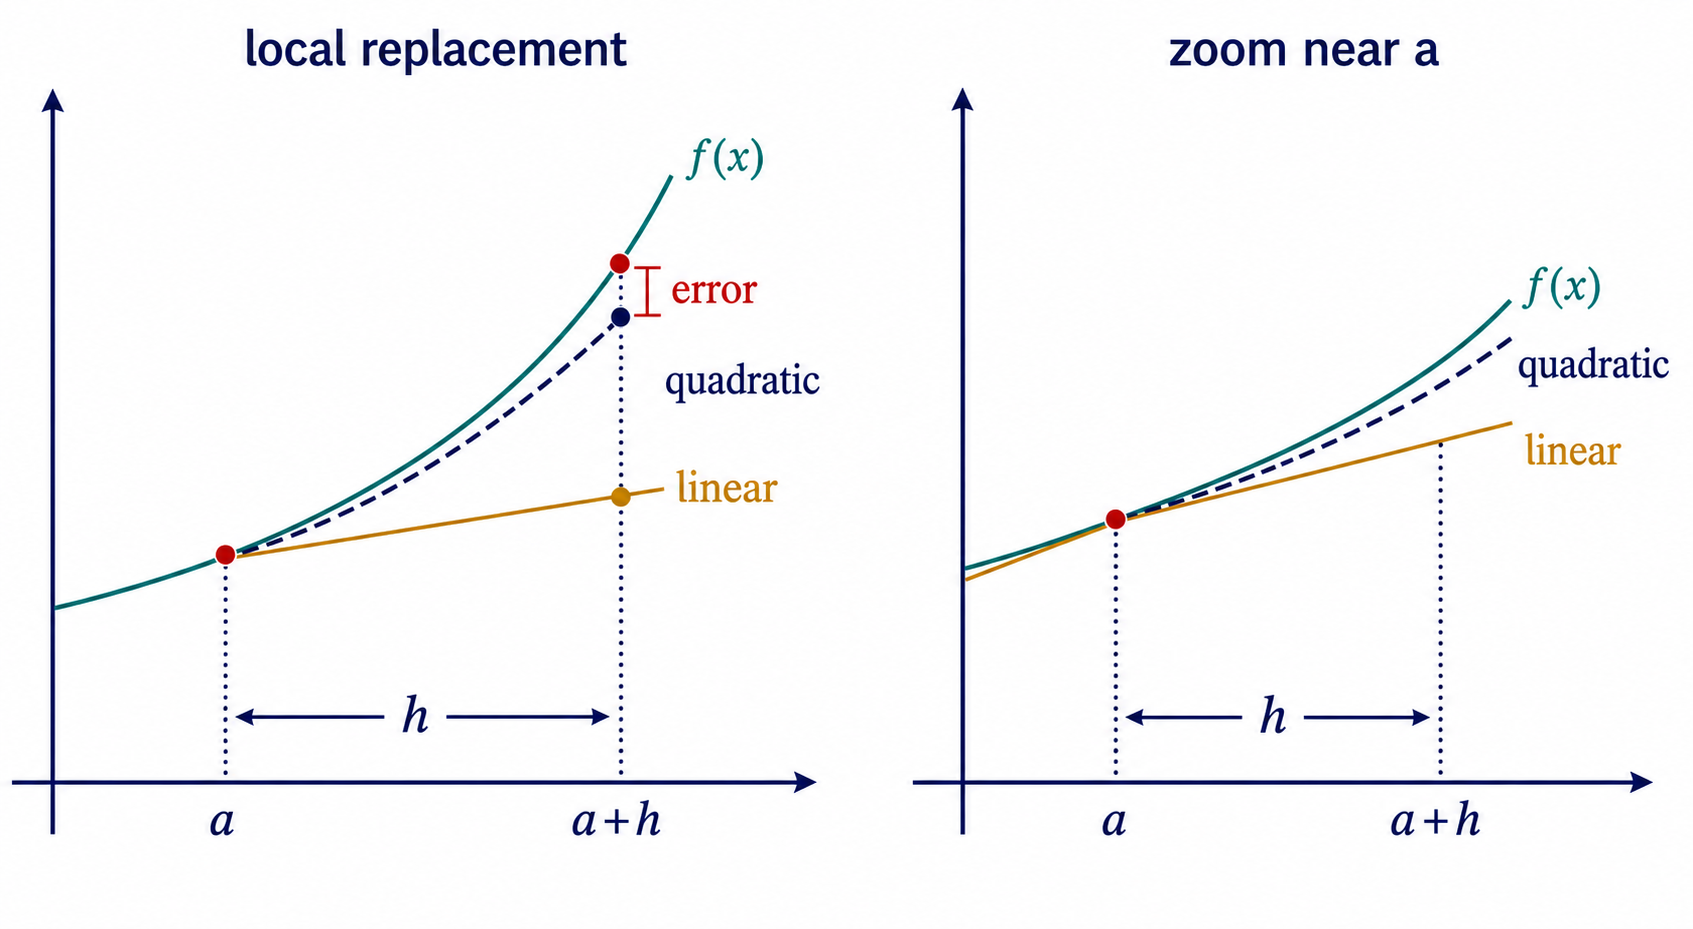
\includegraphics[width=0.95\linewidth]{imagegen-figures/ch10-taylor-local-models-v2.png}
\caption{Taylor approximation replaces a nonlinear function by a local model near a base point. The first-order model uses the tangent line, while the second-order model also uses curvature. For small \(h\), the quadratic model typically leaves a smaller local error than the linear model.}
\label{fig:ch10-taylor-local-models}
\end{figure}

\paragraph{Formal setup.}
Let \(f:I\to\mathbb{R}\) have \(k\) derivatives near an interior point \(a\in I\). The degree-\(k\) Taylor polynomial of \(f\) around \(a\) is
\[
P_k(a+h)=
\sum_{j=0}^k \frac{f^{(j)}(a)}{j!}h^j
=
f(a)+f'(a)h+\frac{f''(a)}{2!}h^2+\cdots+\frac{f^{(k)}(a)}{k!}h^k.
\]
The function value is written as
\[
f(a+h)=P_k(a+h)+R_k(h),
\]
where \(R_k(h)\) is the remainder. Under appropriate smoothness assumptions, \(R_k(h)\) is small compared with \(h^k\) in a precise way.

For a scalar-valued multivariable function \(f:U\subseteq\mathbb{R}^n\to\mathbb{R}\) with continuous second partial derivatives near \(a\), the central second-order Taylor model is
\[
f(a+h)
=
f(a)+\nabla f(a)^\top h+\frac{1}{2}h^\top H_f(a)h+R_2(h),
\qquad
\frac{R_2(h)}{\|h\|_2^2}\to 0
\quad\text{as }h\to0.
\]
Here \(h\in\mathbb{R}^n\), \(\nabla f(a)\in\mathbb{R}^n\), and \(H_f(a)\in\mathbb{R}^{n\times n}\). The linear term records slope; the quadratic term records curvature.

\paragraph{Core intuition.}
Figure~\ref{fig:ch10-taylor-local-models} shows the replacement idea. At the base point \(a\), the function, tangent model, and quadratic model share the same value. The tangent model also shares the same slope. The quadratic model additionally shares the same local curvature, so it often tracks the nonlinear curve better over a small neighborhood.

The multivariable version says the same thing in vector language. The displacement \(h\) is a proposed local move. The dot product \(\nabla f(a)^\top h\) predicts first-order change in that direction. The quadratic form \(h^\top H_f(a)h\) corrects the prediction using curvature along \(h\). This is why gradients and Hessians from Chapter 9 were not isolated derivative symbols: together they are coefficients of a local model.

Two beginner misconceptions are common. First, a Taylor polynomial does not automatically converge to the function far away from the base point. Some Taylor series have limited radii of convergence, and finite Taylor polynomials always have scale-dependent error. Second, a second-order model is not always better for every displacement. It is usually better sufficiently close to the base point when the required derivatives behave well.

This section connects backward to Chapter 8's local linearization and Chapter 9's Hessian curvature. It connects forward to optimization, Laplace approximations, local stability analysis, and differential geometry, where local replacements are the basic currency.

\paragraph{Main derivation: matching derivatives determines the quadratic model.}
Suppose we want a quadratic polynomial
\[
q(h)=c_0+c_1h+c_2h^2
\]
to match \(f(a+h)\) at \(h=0\) through second order. Matching the value gives
\[
q(0)=c_0=f(a).
\]
Matching the first derivative with respect to \(h\) gives
\[
q'(h)=c_1+2c_2h,
\qquad
q'(0)=c_1=f'(a).
\]
Matching the second derivative gives
\[
q''(h)=2c_2,
\qquad
q''(0)=2c_2=f''(a),
\]
so \(c_2=f''(a)/2\). Therefore
\[
q(h)=f(a)+f'(a)h+\frac{1}{2}f''(a)h^2.
\]
The factorial \(2!\) appears because differentiating \(h^2\) twice produces the factor \(2\).

For the multivariable model, restrict \(f\) to a line through \(a\) in direction \(h\):
\[
g(t)=f(a+t h).
\]
Applying the one-variable quadratic approximation to \(g\) near \(t=0\) gives
\[
g(1)\approx g(0)+g'(0)+\frac{1}{2}g''(0).
\]
By the chain rule,
\[
g'(0)=\nabla f(a)^\top h,
\qquad
g''(0)=h^\top H_f(a)h.
\]
Since \(g(1)=f(a+h)\), we obtain
\[
f(a+h)\approx f(a)+\nabla f(a)^\top h+\frac{1}{2}h^\top H_f(a)h.
\]

\paragraph{Worked examples.}
\emph{Small numerical example.} Approximate \(\sqrt{1+h}\) near \(h=0\). Let \(f(x)=\sqrt{x}\), \(a=1\), and write \(x=1+h\). Then
\[
f(1)=1,\qquad f'(x)=\frac{1}{2\sqrt{x}},\qquad f'(1)=\frac{1}{2},
\]
and
\[
f''(x)=-\frac{1}{4x^{3/2}},
\qquad
f''(1)=-\frac{1}{4}.
\]
The quadratic Taylor approximation is
\[
\sqrt{1+h}\approx 1+\frac{1}{2}h-\frac{1}{8}h^2.
\]
For \(h=0.2\), this gives \(1+0.1-0.005=1.095\). The exact value is \(\sqrt{1.2}\approx1.09545\).

\emph{ML/neuroscience example.} Consider a scalar loss \(L(\theta)\) near a trained parameter vector \(\hat{\theta}\). A local perturbation \(h\) changes the loss approximately by
\[
L(\hat{\theta}+h)-L(\hat{\theta})
\approx
\nabla L(\hat{\theta})^\top h+\frac{1}{2}h^\top H_L(\hat{\theta})h.
\]
If training has made \(\nabla L(\hat{\theta})\approx0\), the Hessian term predicts which parameter directions are sensitive. In a neural population model, if \(r(s)\) is the firing rate as a function of stimulus \(s\), a Taylor model near \(s_0\) predicts how small stimulus perturbations change the rate without refitting the full nonlinear response curve.

\paragraph{ML/DL/neuroscience connections.}
In deep learning, Taylor approximations support loss-landscape analysis, adversarial perturbation analysis, pruning criteria, and second-order optimization. The function \(f\) becomes a loss \(L\), the base point \(a\) becomes the current parameter vector \(\theta_0\), and \(h\) becomes a candidate parameter or input perturbation. In neuroscience, local Taylor models approximate nonlinear tuning curves, local input-output gains, and energy landscapes near equilibria. In probabilistic modeling, a second-order Taylor approximation of a log likelihood near its maximum becomes the local Gaussian approximation used by Laplace methods.

\paragraph{Exercises.}
\begin{enumerate}[label=\textbf{10.1.\arabic*.}, leftmargin=*]
\item \textbf{Mechanical.} Find the second-order Taylor approximation of \(\cos x\) around \(a=0\). Use it to approximate \(\cos(0.2)\).
\item \textbf{Proof or derivation.} Derive the quadratic Taylor model for a one-variable function by matching value, first derivative, and second derivative at \(h=0\), as in the section.
\item \textbf{Numerical/computational.} For \(f(x)=\log(1+x)\), compare the first-order and second-order Taylor approximations at \(x=0.1\), \(0.5\), and \(1.0\). Which errors grow fastest?
\item \textbf{Interpretation.} In the local model \(L(\theta_0+h)\approx L(\theta_0)+\nabla L(\theta_0)^\top h+\frac{1}{2}h^\top H_L(\theta_0)h\), what do the two terms involving \(h\) say about a parameter perturbation?
\item \textbf{Debug the misconception.} A student says, "The Taylor polynomial is the same thing as the function." Correct the statement and explain what local information the polynomial preserves.
\end{enumerate}

\subsection{10.2 Local geometry of optimization landscapes}

\paragraph{Motivating question.}
Near the current parameter vector, how do gradients and Hessians reveal descent directions, minima, saddles, flat directions, and conditioning?

\paragraph{Beginner setup.}
An optimization landscape is a scalar-valued function viewed over its input space. In machine learning the function is often a loss
\[
L:\mathbb{R}^p\to\mathbb{R},
\]
where \(\theta\in\mathbb{R}^p\) is the parameter vector. Taylor approximation says that near a current point \(\theta_0\),
\[
L(\theta_0+h)\approx
L(\theta_0)+g^\top h+\frac{1}{2}h^\top Hh,
\]
where \(g=\nabla L(\theta_0)\) and \(H=H_L(\theta_0)\).

The smallest clear example is
\[
L(x,y)=x^2+10y^2.
\]
At \((0,0)\), the gradient is zero and
\[
H=
\begin{bmatrix}
2&0\\
0&20
\end{bmatrix}.
\]
The point is a local minimum, but the curvature in the \(y\)-direction is ten times larger than the curvature in the \(x\)-direction. Contours are narrow ellipses, and gradient descent must respect the steep direction to avoid overshooting.

This concept solves the diagnostic problem of optimization. The gradient says where the loss decreases first. The Hessian says how the slope changes, whether a critical point is a minimum or saddle, and whether the landscape is well-conditioned or stretched into a long valley.

What to keep in mind: optimization is local before it is global. The Taylor model describes a neighborhood of \(\theta_0\). It cannot by itself prove that a nonconvex model has no better minimum elsewhere.

\begin{figure}[htbp]
\centering
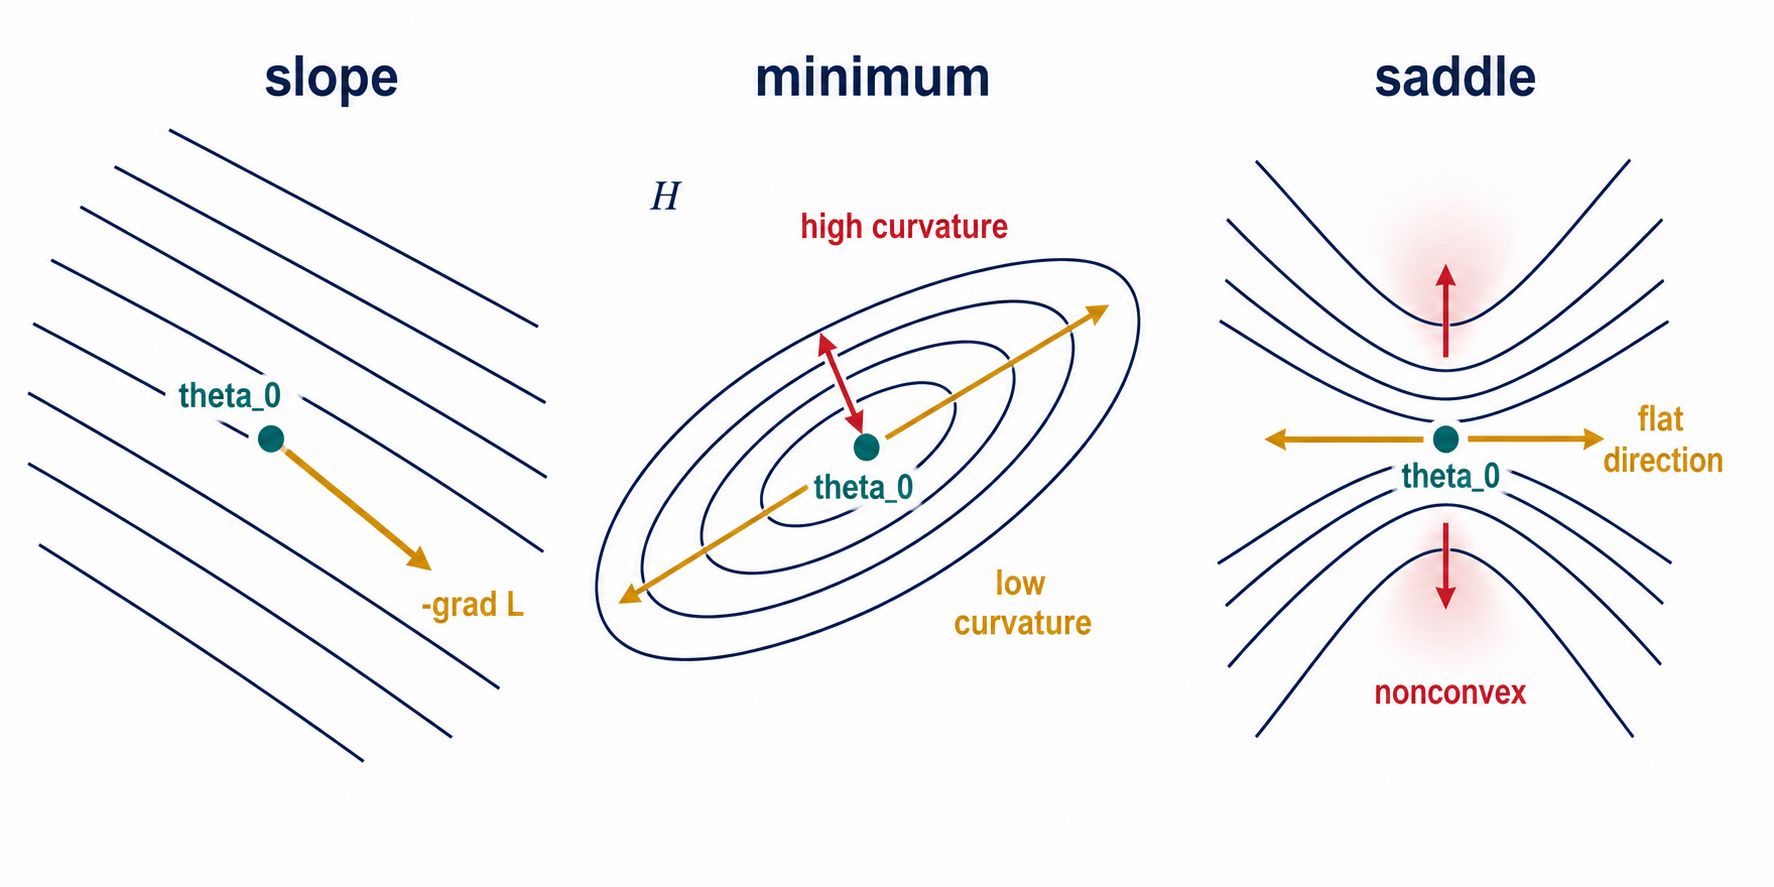
\includegraphics[width=0.96\linewidth]{imagegen-figures/ch10-optimization-local-geometry.png}
\caption{Local optimization geometry comes from the Taylor model of a loss. Away from a critical point, the gradient gives the first-order descent direction. Near a minimum, Hessian eigenvectors show high- and low-curvature directions. Near a saddle or flat region, the same local model reveals directions that can be unstable, slow, or nearly unchanged.}
\label{fig:ch10-optimization-local-geometry}
\end{figure}

\paragraph{Formal setup.}
Let \(L:U\subseteq\mathbb{R}^p\to\mathbb{R}\) have continuous second partial derivatives near \(\theta_0\). Define
\[
g=\nabla L(\theta_0)\in\mathbb{R}^p,
\qquad
H=H_L(\theta_0)\in\mathbb{R}^{p\times p}.
\]
The local quadratic model is
\[
m_{\theta_0}(h)
=
L(\theta_0)+g^\top h+\frac{1}{2}h^\top Hh.
\]
The eigenvectors of the symmetric Hessian \(H\) are local curvature directions. If \(Hv_i=\lambda_i v_i\) and \(\|v_i\|_2=1\), then the quadratic curvature along \(v_i\) is \(\lambda_i\):
\[
m_{\theta_0}(t v_i)-L(\theta_0)
=
t\,g^\top v_i+\frac{1}{2}\lambda_i t^2.
\]

If \(g=0\), the point \(\theta_0\) is a critical point. If all eigenvalues of \(H\) are positive, the local model is a bowl. If some eigenvalues are positive and others negative, the local model is a saddle. If positive eigenvalues differ greatly in size, the local bowl is ill-conditioned. For a positive definite Hessian, a basic condition number is
\[
\kappa(H)=\frac{\lambda_{\max}(H)}{\lambda_{\min}(H)}.
\]
Large \(\kappa(H)\) means very different curvature scales in different directions.

\paragraph{Core intuition.}
Figure~\ref{fig:ch10-optimization-local-geometry} shows three local views. When \(g\neq0\), the linear term \(g^\top h\) dominates very small steps, so \(-g\) is the steepest first-order descent direction under the Euclidean norm. At a well-behaved minimum, the gradient is zero and the Hessian is positive definite, so the contours close around the point. In a saddle region, some directions curve up while others curve down or remain nearly flat.

Conditioning is geometry, not just a numerical nuisance. In a circular bowl, the same step size can work in all directions. In a narrow valley, a step size small enough for the steep direction may make slow progress along the flat direction. This is why rescaling, normalization, momentum, adaptive methods, and second-order approximations matter in training.

Common misconceptions: a zero gradient does not imply a good solution; it may be a saddle. A small training loss does not imply a sharp or stable minimum; flat directions may allow many nearby parameter settings with similar predictions. Convex local geometry also does not imply global convexity unless the function is convex over the whole relevant domain.

This section uses Taylor approximation from Section 10.1 and Hessian eigenvalue geometry from Chapters 6 and 9. It prepares Newton methods, natural gradients, Fisher information, local Gaussian approximations, and the analysis of high-dimensional nonconvex losses.

\paragraph{Main derivation: the Newton step from the local quadratic model.}
Assume \(H\) is invertible and use the local model
\[
m_{\theta_0}(h)=L(\theta_0)+g^\top h+\frac{1}{2}h^\top Hh.
\]
To minimize this quadratic model with respect to \(h\), differentiate with respect to \(h\):
\[
\nabla_h m_{\theta_0}(h)=g+Hh.
\]
Setting this model-gradient equal to zero gives
\[
g+Hh=0.
\]
If \(H\) is invertible, the stationary step is
\[
h_\star=-H^{-1}g.
\]
Thus Newton's update is
\[
\theta_{\text{new}}=\theta_0-H^{-1}\nabla L(\theta_0).
\]
When \(H\) is positive definite and the Taylor model is accurate, this step moves to the minimizer of the local quadratic model. When \(H\) is indefinite or the model is inaccurate far from \(\theta_0\), the same algebra can point toward unstable directions, so practical methods use damping, trust regions, or curvature approximations.

\paragraph{Worked examples.}
\emph{Small numerical example.} Let
\[
L(x,y)=\frac{1}{2}(4x^2+y^2).
\]
At \(\theta_0=(1,1)^\top\),
\[
g=
\begin{bmatrix}
4\\
1
\end{bmatrix},
\qquad
H=
\begin{bmatrix}
4&0\\
0&1
\end{bmatrix}.
\]
A gradient step with \(\eta=0.1\) gives
\[
\theta_1=\theta_0-\eta g=(1,1)^\top-0.1(4,1)^\top=(0.6,0.9)^\top.
\]
The Newton step is
\[
h_\star=-H^{-1}g=-(1,1)^\top,
\]
so it moves directly to \((0,0)\), the minimum of this exact quadratic. The difference occurs because Newton rescales the gradient by curvature.

\emph{ML/neuroscience example.} In a deep network, \(L(\theta)\) may have millions of coordinates. Around a trained \(\hat{\theta}\), many Hessian eigenvalues can be close to zero. Those eigenvectors represent parameter directions where the network's training loss changes little. In a neural energy model \(E(x)\), a stable attractor corresponds locally to a positive curvature basin. Saddle directions indicate ways a neural state can leave one basin and move toward another state pattern.

\paragraph{ML/DL/neuroscience connections.}
In deep learning, the Hessian is often too large to form explicitly, but Hessian-vector products estimate curvature along chosen directions. Sharpness analysis studies large positive eigenvalues of \(H_L(\hat{\theta})\); flatness analysis studies small eigenvalues and low-loss directions. In recurrent networks and theoretical neuroscience, energy landscapes use the same local geometry: the state vector \(x\) replaces the parameter vector \(\theta\), and the energy \(E(x)\) replaces the loss \(L(\theta)\). In probabilistic inference, the negative Hessian of a log posterior near a mode gives a local uncertainty shape.

\paragraph{Exercises.}
\begin{enumerate}[label=\textbf{10.2.\arabic*.}, leftmargin=*]
\item \textbf{Mechanical.} For \(L(x,y)=x^2+5y^2\), compute \(\nabla L\), \(H_L\), the Hessian eigenvalues, and the condition number.
\item \textbf{Proof or derivation.} Starting from \(m(h)=L(\theta_0)+g^\top h+\frac{1}{2}h^\top Hh\), derive the Newton step \(h_\star=-H^{-1}g\) when \(H\) is invertible.
\item \textbf{Numerical/computational.} For \(L(x,y)=\frac{1}{2}(100x^2+y^2)\), take one gradient-descent step from \((1,1)\) with \(\eta=0.01\). Explain why a much larger step size would be dangerous in the \(x\)-direction.
\item \textbf{Interpretation.} A model has near-zero gradient at \(\hat{\theta}\), but the Hessian has both positive and negative eigenvalues. What does this say about the local landscape?
\item \textbf{Debug the misconception.} A student says, "If the loss is locally convex near \(\theta_0\), then \(\theta_0\) is globally optimal." Explain what local Taylor geometry can and cannot prove.
\end{enumerate}

\subsection{10.3 Manifolds as locally flat spaces}

\paragraph{Motivating question.}
How can a curved space be studied with linear tools if it looks flat only near each point?

\paragraph{Beginner setup.}
A manifold is a space that may be curved globally but resembles ordinary Euclidean space in small neighborhoods. A circle is not a line globally, but a tiny arc of a circle looks like a line. A sphere is not a plane globally, but a tiny patch of a sphere looks like a plane.

The smallest example is the unit circle
\[
S^1=\{(x,y)\in\mathbb{R}^2:x^2+y^2=1\}.
\]
Near most points, a small arc can be described by one coordinate, such as an angle \(t\). The map
\[
\psi(t)=(\cos t,\sin t)
\]
turns the coordinate \(t\) into a point on the circle. Differentiating gives
\[
\psi'(t)=(-\sin t,\cos t),
\]
which is a tangent vector along the circle.

Manifolds solve the modeling problem created by intrinsically low-dimensional but curved spaces. Neural population activity may live near a low-dimensional curved set inside a high-dimensional recording space. A robot arm's configurations may form a curved space of joint angles. Normalized vectors live on spheres; probability vectors live on simplexes.

What to keep in mind: a manifold is not usually a vector space. You cannot freely add two points on a sphere and expect to remain on the sphere. Linear operations belong in tangent spaces, which approximate the manifold near a point.

\begin{figure}[htbp]
\centering
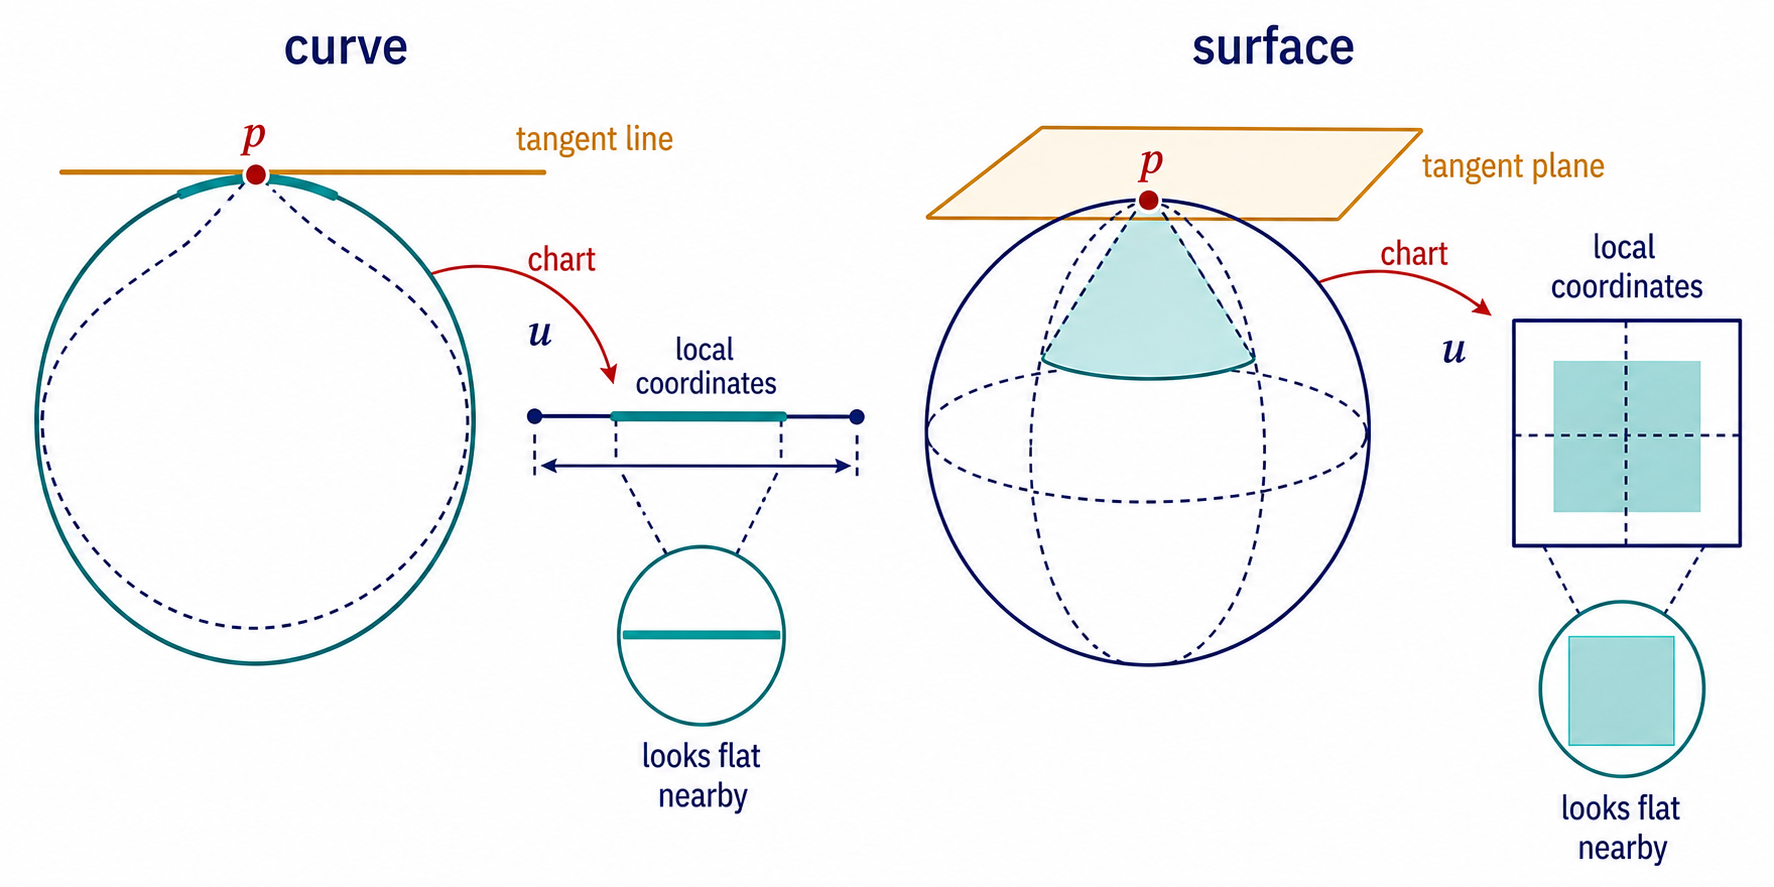
\includegraphics[width=0.96\linewidth]{imagegen-figures/ch10-manifold-local-charts.png}
\caption{A manifold can be curved globally while looking flat nearby. A chart assigns local coordinates to a small patch, and the tangent line or tangent plane gives the best local linear space at a point \(p\). Calculus on manifolds works by moving between curved patches and local coordinates.}
\label{fig:ch10-manifold-local-charts}
\end{figure}

\paragraph{Formal setup.}
Informally, a \(d\)-dimensional manifold \(M\) is a space where each point \(p\in M\) has a neighborhood that can be coordinatized by an open subset of \(\mathbb{R}^d\). A chart is a map
\[
\phi:V\subset M\to U\subset\mathbb{R}^d
\]
that assigns local coordinates to points in a neighborhood \(V\) of \(p\). The inverse map, when written as a local parameterization,
\[
\psi:U\subset\mathbb{R}^d\to M\subset\mathbb{R}^n,
\]
takes coordinates \(u\in\mathbb{R}^d\) and returns points in the ambient space \(\mathbb{R}^n\).

For an embedded manifold parameterized by \(\psi\), the tangent space at \(p=\psi(u_0)\) is spanned by the columns of the Jacobian:
\[
T_pM=\operatorname{span}\left\{
\frac{\partial \psi}{\partial u_1}(u_0),\ldots,
\frac{\partial \psi}{\partial u_d}(u_0)
\right\}.
\]
Equivalently, tangent vectors are velocities of curves that stay on the manifold:
\[
T_pM=\{\gamma'(0):\gamma(t)\in M,\ \gamma(0)=p\}.
\]
The dimension of \(T_pM\) is \(d\) at regular points.

\paragraph{Core intuition.}
Figure~\ref{fig:ch10-manifold-local-charts} shows the main idea. The circle and sphere are curved, so no single flat coordinate system describes them perfectly everywhere without distortion or singularities. But near a point \(p\), a small arc or patch can be flattened into coordinates. The tangent space is the best linear approximation to the manifold at that point.

Charts are like local maps of a city. A paper map can represent a neighborhood well even if it cannot represent the whole earth without distortion. When a model learns a latent coordinate \(z\) and decodes it to a high-dimensional activity vector \(x=\psi(z)\), the decoder is a parameterization of a learned representation manifold. Its Jacobian tells how latent moves change observable activity.

Common misconceptions: a manifold need not be a surface in three-dimensional space; it can live in very high-dimensional space. A tangent space touches the manifold locally but is not the same as the manifold. A chart is not the manifold itself; it is a coordinate description of a patch. Finally, global curvature does not prevent local linear approximation.

This section connects Taylor approximation to geometry. Taylor's first-order term is a tangent-line or tangent-plane model for functions. A manifold's tangent space is the corresponding local linear model for a space. Later chapters use this idea for latent manifolds, neural state spaces, normalizing flows, and information geometry.

\paragraph{Main derivation: tangent space to the circle.}
Let
\[
S^1=\{p=(x,y)^\top\in\mathbb{R}^2:x^2+y^2=1\}.
\]
Suppose \(\gamma(t)\) is a differentiable curve on the circle with \(\gamma(0)=p\). Since \(\gamma(t)\in S^1\), it satisfies
\[
\|\gamma(t)\|_2^2=1
\]
for all \(t\). Differentiate both sides at \(t=0\):
\[
\frac{d}{dt}\left(\gamma(t)^\top\gamma(t)\right)\bigg|_{t=0}=0.
\]
Using the product rule gives
\[
2\gamma(0)^\top\gamma'(0)=0.
\]
Since \(\gamma(0)=p\), any tangent velocity \(v=\gamma'(0)\) must satisfy
\[
p^\top v=0.
\]
Therefore
\[
T_pS^1=\{v\in\mathbb{R}^2:p^\top v=0\}.
\]
The tangent line consists of all directions perpendicular to the radius vector \(p\). This derivation teaches the mechanism: differentiate the constraint that defines the manifold, and the derivative gives the allowable infinitesimal directions.

\paragraph{Worked examples.}
\emph{Small symbolic example.} At the point
\[
p=(1,0)^\top\in S^1,
\]
the tangent space is
\[
T_pS^1=\{v=(v_1,v_2)^\top:(1,0)\cdot(v_1,v_2)=0\}
=\{(0,v_2)^\top:v_2\in\mathbb{R}\}.
\]
So the tangent line is vertical. At
\[
p=\frac{1}{\sqrt{2}}(1,1)^\top,
\]
the tangent vectors satisfy \(v_1+v_2=0\), so one tangent direction is \((1,-1)^\top\).

\emph{ML/neuroscience example.} Suppose a two-dimensional latent variable \(z=(z_1,z_2)\) is decoded into a neural population response \(r=\psi(z)\in\mathbb{R}^{100}\). The set of possible responses
\[
M=\{\psi(z):z\in\mathbb{R}^2\}
\]
is a two-dimensional manifold inside a 100-dimensional recording space, at least where \(J_\psi(z)\) has rank \(2\). The two columns of \(J_\psi(z)\) span the tangent plane: they are the population activity changes caused by small moves in each latent coordinate. This maps the mathematical tangent basis to experimentally observable population-change directions.

\paragraph{ML/DL/neuroscience connections.}
Data often concentrate near lower-dimensional manifolds. The ambient coordinates may be pixels, neural firing rates, hidden activations, or behavioral measurements; the local coordinates may be latent variables. In deep generative models, a decoder \(\psi(z)\) maps latent coordinates to data, and its Jacobian spans local directions of variation. In neuroscience, low-dimensional neural manifolds summarize population states during reaching, navigation, decision making, or memory. Tangent spaces then describe local neural state changes rather than arbitrary directions in the full neuron space.

\paragraph{Exercises.}
\begin{enumerate}[label=\textbf{10.3.\arabic*.}, leftmargin=*]
\item \textbf{Mechanical.} For the circle parameterization \(\psi(t)=(\cos t,\sin t)\), compute \(\psi'(0)\) and \(\psi'(\pi/2)\). Interpret each tangent vector geometrically.
\item \textbf{Proof or derivation.} Use the constraint \(x^2+y^2+z^2=1\) to show that the tangent space to the unit sphere at \(p\in S^2\) is \(T_pS^2=\{v\in\mathbb{R}^3:p^\top v=0\}\).
\item \textbf{Numerical/computational.} Let \(\psi(z)=(z,z^2,z^3)^\top\). Compute the tangent vector \(J_\psi(2)\) and use it to approximate \(\psi(2.01)-\psi(2)\).
\item \textbf{Interpretation.} In a neural manifold model \(r=\psi(z)\), what do the columns of \(J_\psi(z)\) mean in terms of population activity?
\item \textbf{Debug the misconception.} A student says, "Because a sphere has tangent planes, it must be a plane." Explain why tangent spaces are local approximations, not global identities.
\end{enumerate}

\subsection{10.4 Constrained surfaces and Lagrange geometry}

\paragraph{Motivating question.}
When an optimum must stay on a constrained surface, why do the objective gradient and constraint gradient become aligned?

\paragraph{Beginner setup.}
In unconstrained optimization, a local optimum usually has zero gradient. In constrained optimization, the gradient of the objective need not be zero, because many directions are not allowed. If the feasible set is
\[
M=\{x\in\mathbb{R}^n:g(x)=0\},
\]
then allowable infinitesimal moves at a regular point \(p\) lie in the tangent space to the constraint surface. For one constraint,
\[
T_pM=\{v\in\mathbb{R}^n:\nabla g(p)^\top v=0\},
\]
provided \(\nabla g(p)\neq0\).

The smallest example is optimizing a linear function on the unit circle:
\[
\text{maximize } f(x,y)=x+2y
\quad\text{subject to}\quad
g(x,y)=x^2+y^2-1=0.
\]
The unconstrained objective increases forever in direction \((1,2)\), but the circle only permits points of unit length. The optimum occurs where the circle point points in the same direction as \((1,2)\).

What to keep in mind: constrained optimality means no allowed first-order move improves the objective. It does not mean \(\nabla f=0\) in the ambient space. It means the tangent component of \(\nabla f\) vanishes.

\begin{figure}[htbp]
\centering
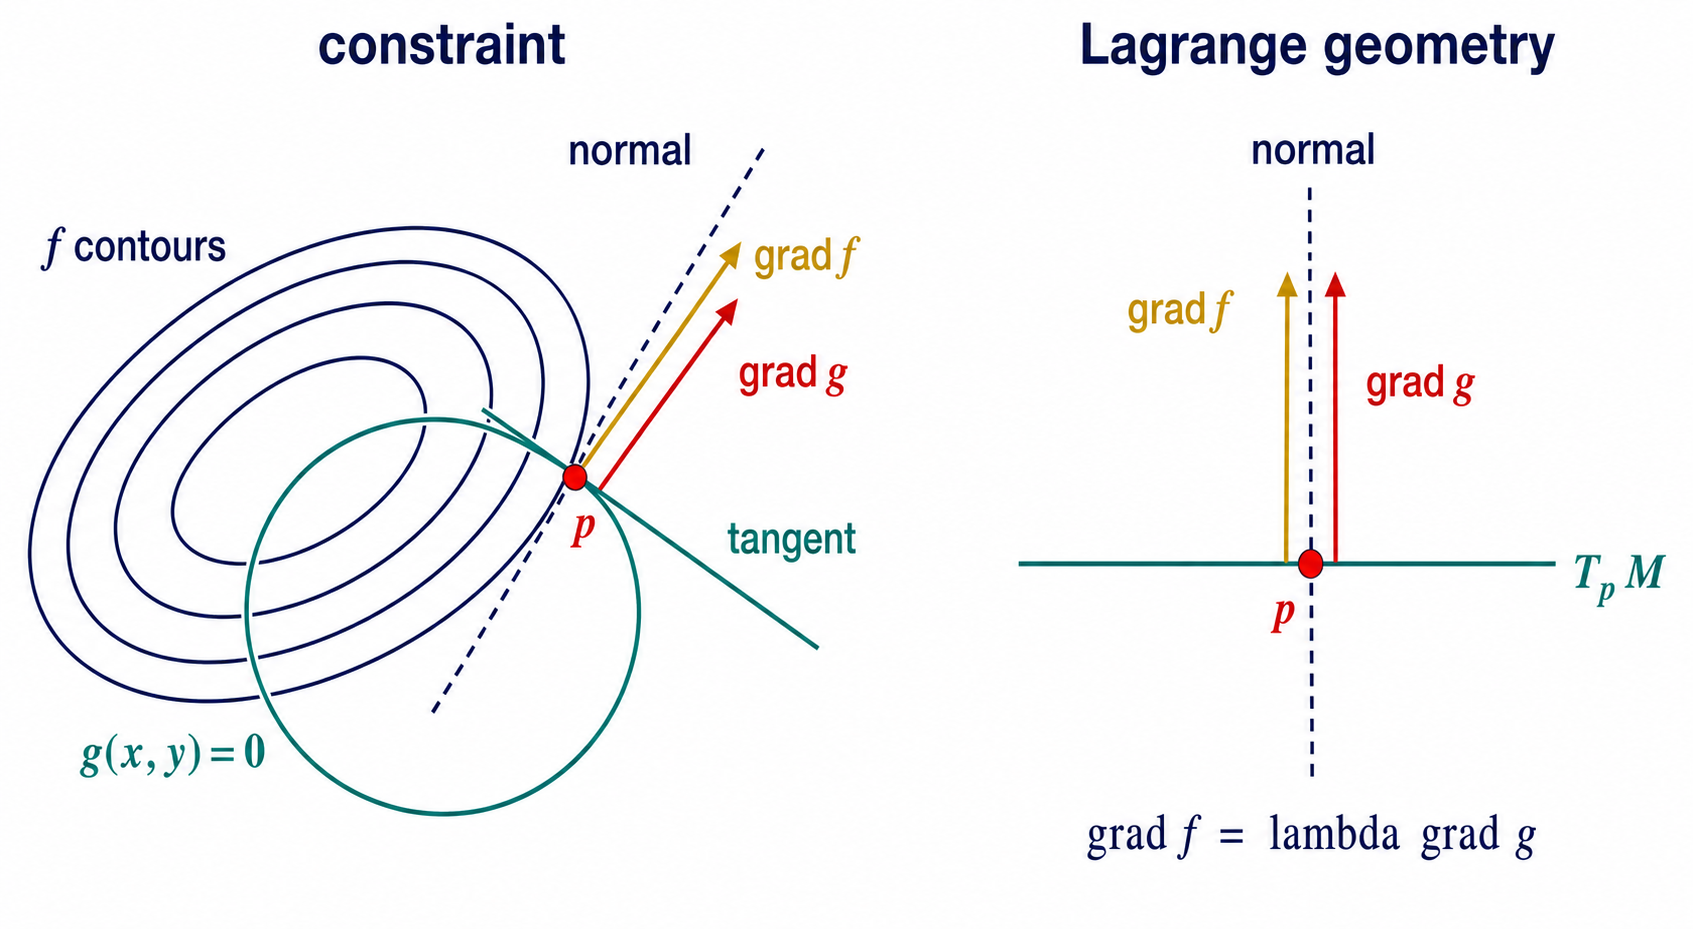
\includegraphics[width=0.96\linewidth]{imagegen-figures/ch10-lagrange-constraint-geometry.png}
\caption{At a constrained optimum, the objective contour is tangent to the feasible surface. The tangent direction gives allowed first-order moves, while \(\nabla g\) is normal to the constraint. If no tangent move can improve \(f\), then \(\nabla f\) has no tangent component, so it lies in the normal direction: \(\nabla f=\lambda\nabla g\).}
\label{fig:ch10-lagrange-constraint-geometry}
\end{figure}

\paragraph{Formal setup.}
Let \(f\) and \(g\) be continuously differentiable maps from \(\mathbb{R}^n\) to \(\mathbb{R}\). Consider the equality-constrained problem
\[
\text{optimize } f(x)
\qquad
\text{subject to}\qquad
g(x)=0.
\]
Assume \(p\) is a local constrained optimum and \(\nabla g(p)\neq0\). The Lagrange multiplier condition says there exists a scalar \(\lambda\in\mathbb{R}\) such that
\[
\nabla f(p)=\lambda \nabla g(p),
\qquad
g(p)=0.
\]
Equivalently, define the Lagrangian
\[
\mathcal{L}(x,\lambda)=f(x)-\lambda g(x).
\]
The first-order conditions are
\[
\nabla_x\mathcal{L}(p,\lambda)=0,
\qquad
\frac{\partial \mathcal{L}}{\partial \lambda}(p,\lambda)=0.
\]
For multiple equality constraints \(g_1(x)=0,\ldots,g_m(x)=0\), the corresponding condition is
\[
\nabla f(p)=\sum_{i=1}^m \lambda_i \nabla g_i(p),
\]
assuming the constraint gradients are independent at \(p\).

\paragraph{Core intuition.}
Figure~\ref{fig:ch10-lagrange-constraint-geometry} shows the geometry. The constraint \(g(x)=0\) is the feasible surface. At a regular point, \(\nabla g(p)\) points normal to that surface because moving tangent to a level set of \(g\) produces no first-order change in \(g\). If \(p\) is an optimum on the surface, every feasible tangent direction \(v\in T_pM\) must satisfy
\[
\nabla f(p)^\top v=0.
\]
So \(\nabla f(p)\) is also normal to the feasible surface. With one constraint, the normal space is the line spanned by \(\nabla g(p)\), so the two gradients are parallel.

A beginner misconception is that Lagrange multipliers are magic algebraic tricks. They are bookkeeping for tangent and normal geometry. Another misconception is that \(\lambda\) is always a penalty weight. In the first-order condition, \(\lambda\) is a multiplier that records how much constraint-normal direction is needed to match the objective gradient. Penalty methods are related but different algorithms.

Constraint qualifications matter. If \(\nabla g(p)=0\), the constraint may have a singular point, and the simple tangent/normal argument can fail. Inequality constraints add another layer because inactive constraints do not affect the local tangent space, while active constraints do. This chapter keeps the equality-constrained regular case as the geometric foundation.

This section connects backward to manifolds as constraint surfaces and forward to optimization with norm constraints, probability simplexes, constrained latent variables, and projected-gradient algorithms.

\paragraph{Main derivation: Lagrange condition from tangent directions.}
Let \(M=\{x:g(x)=0\}\), and let \(p\in M\) be a regular constrained local optimum. Any differentiable feasible curve \(\gamma(t)\in M\) with \(\gamma(0)=p\) has tangent velocity \(v=\gamma'(0)\in T_pM\). Because \(p\) is a constrained optimum of \(f\), the one-variable function
\[
\ell(t)=f(\gamma(t))
\]
has a local optimum at \(t=0\), so
\[
\ell'(0)=0.
\]
By the chain rule,
\[
\ell'(0)=\nabla f(p)^\top \gamma'(0)=\nabla f(p)^\top v.
\]
Thus \(\nabla f(p)^\top v=0\) for every tangent vector \(v\in T_pM\).

For one regular constraint, differentiating \(g(\gamma(t))=0\) gives
\[
\nabla g(p)^\top v=0,
\]
so
\[
T_pM=\{v:\nabla g(p)^\top v=0\}.
\]
The vectors orthogonal to this tangent space form the normal line \(\operatorname{span}\{\nabla g(p)\}\). Since \(\nabla f(p)\) is orthogonal to every tangent vector, it lies in this normal line. Therefore there is a scalar \(\lambda\) such that
\[
\nabla f(p)=\lambda\nabla g(p).
\]

\paragraph{Worked examples.}
\emph{Small numerical example.} Maximize
\[
f(x,y)=x+2y
\]
subject to
\[
g(x,y)=x^2+y^2-1=0.
\]
The gradients are
\[
\nabla f=
\begin{bmatrix}
1\\
2
\end{bmatrix},
\qquad
\nabla g=
\begin{bmatrix}
2x\\
2y
\end{bmatrix}.
\]
The Lagrange condition \(\nabla f=\lambda\nabla g\) gives
\[
1=2\lambda x,
\qquad
2=2\lambda y.
\]
Thus \(y=2x\). The constraint gives
\[
x^2+(2x)^2=1,
\qquad
5x^2=1.
\]
The maximum is at
\[
(x,y)=\left(\frac{1}{\sqrt{5}},\frac{2}{\sqrt{5}}\right),
\]
where \(f=\sqrt{5}\). The minimum is the opposite point, with value \(-\sqrt{5}\).

\emph{ML/neuroscience example.} In a classifier, a probability vector \(p=(p_1,\ldots,p_K)\) must satisfy
\[
\sum_{i=1}^K p_i=1,
\qquad
p_i\geq0.
\]
If we temporarily ignore the inequality boundaries and optimize an objective over the equality constraint \(\sum_i p_i=1\), the feasible tangent directions \(v\) satisfy \(\sum_i v_i=0\). Lagrange geometry says that at an interior constrained optimum, the objective gradient can differ across coordinates only through the normal direction to the simplex constraint. In neural modeling, firing-rate vectors with fixed total activity satisfy a similar normalization constraint; allowed perturbations redistribute activity without changing the total.

\paragraph{ML/DL/neuroscience connections.}
Constrained optimization appears whenever model parameters, states, or predictions must satisfy structure. Norm-constrained embeddings lie on spheres. Probability vectors lie on simplexes. Orthogonal weight matrices lie on matrix manifolds. Low-rank factors may be identifiable only up to rotations or scalings. In each case, the ambient gradient must be converted into an allowed direction, either through Lagrange equations, projected gradients, or manifold optimization. In neuroscience, constrained latent-state models can enforce fixed energy, fixed total firing rate, or normalized population activity; the tangent space describes feasible instantaneous changes in the state.

\paragraph{Exercises.}
\begin{enumerate}[label=\textbf{10.4.\arabic*.}, leftmargin=*]
\item \textbf{Mechanical.} Use Lagrange multipliers to maximize \(f(x,y)=3x+y\) subject to \(x^2+y^2=1\). State both the maximum point and maximum value.
\item \textbf{Proof or derivation.} Derive \(T_pM=\{v:\nabla g(p)^\top v=0\}\) by differentiating \(g(\gamma(t))=0\) along a feasible curve \(\gamma(t)\).
\item \textbf{Numerical/computational.} For \(f(x,y)=xy\) constrained to \(x^2+y^2=1\), solve the Lagrange equations and classify the constrained maxima and minima by evaluating \(f\) at the candidate points.
\item \textbf{Interpretation.} For a probability vector constrained by \(\sum_i p_i=1\), what does a feasible tangent perturbation \(v\) have to satisfy, and why?
\item \textbf{Debug the misconception.} A student says, "At every constrained optimum, \(\nabla f=0\)." Use the example \(f(x,y)=x+2y\) on the unit circle to correct the claim.
\end{enumerate}

\paragraph{Closing bridge.}
This chapter made local modeling explicit. Taylor polynomials replace nonlinear functions near a point. Optimization landscapes become local quadratic models whose gradients and Hessians reveal descent, curvature, saddles, and flat directions. Manifolds and constraints show that even the space itself may need local coordinates and tangent spaces before calculus can be used correctly. Chapter 11 carries this local-coordinate viewpoint into integration and change of variables, where Jacobians measure how volumes and densities transform. Later chapters reuse the same ideas for latent representations, neural state spaces, variational inference, information geometry, and constrained learning systems.

\clearpage
